\documentclass[a4paper,12pt]{article}
\usepackage[utf8]{inputenc}
%\usepackage[english]{babel}
\usepackage{amsmath}
\usepackage{amssymb}
\usepackage{amsthm}
\usepackage{geometry}
\usepackage{graphicx}
\usepackage[hidelinks]{hyperref}
\usepackage{listings}
\usepackage{xcolor}
\usepackage{enumitem}
\usepackage{booktabs}
\usepackage{microtype}
\usepackage{natbib}
\usepackage{url}
\usepackage{array}
\usepackage{multirow}

\geometry{
  a4paper,
  left=2.5cm, right=2.5cm,
  top=2.5cm,  bottom=2.5cm
}

% ---- Deutsche Bezeichnungen (ohne babel) ----
\renewcommand{\contentsname}{Inhaltsverzeichnis}
\renewcommand{\listfigurename}{Abbildungsverzeichnis}
\renewcommand{\listtablename}{Tabellenverzeichnis}
\renewcommand{\refname}{Literaturverzeichnis}
\renewcommand{\bibname}{Literaturverzeichnis}
\renewcommand{\figurename}{Abbildung}
\renewcommand{\tablename}{Tabelle}
\renewcommand{\abstractname}{Zusammenfassung}
\renewcommand{\appendixname}{Anhang}
\renewcommand{\proofname}{Beweis}
% Verhindere Zeilenüberlauf
\sloppy
\emergencystretch=2em

\theoremstyle{definition}
\newtheorem{definition}{Definition}[section]
\newtheorem{beispiel}{Beispiel}[section]
\newtheorem{satz}{Satz}[section]
\newtheorem{lemma}{Lemma}[section]
\newtheorem{korollar}{Korollar}[section]
\newtheorem{bemerkung}{Bemerkung}[section]
\newtheorem{proposition}{Proposition}[section]

\setlist[itemize,1]{label=--}

% ---------- Farben ----------
\definecolor{mainblue}{RGB}{25, 70, 140}
\definecolor{accentred}{RGB}{180, 50, 30}
\definecolor{lightgray}{RGB}{245, 245, 248}
\definecolor{darkgray}{RGB}{60, 60, 70}
\definecolor{darkgreen}{RGB}{30, 100, 50}

\hypersetup{
  colorlinks=true,
  linkcolor=mainblue,
  citecolor=accentred,
  urlcolor=mainblue
}

\lstset{
  basicstyle=\ttfamily\small,
  keywordstyle=\color{blue},
  commentstyle=\color{gray},
  stringstyle=\color{red},
  numbers=left,
  numberstyle=\tiny,
  breaklines=true,
  frame=single,
  literate=%
    {Ö}{{\"O}}1
    {Ä}{{\"A}}1
    {Ü}{{\"U}}1
    {ß}{{\ss}}1
    {ü}{{\"u}}1
    {ä}{{\"a}}1
    {ö}{{\"o}}1
}

\title{\textbf{Der Subgraph Algorithmus als strukturelle Erweiterung\\
von LIME: Perturbation, Proximity und Feature-Selektion\\
auf Graphen}}
\author{Stephan Epp}
\date{9. Juni 2026}

\begin{document}

\maketitle
\tableofcontents
\newpage

% ===========================================================
\section{Einführung}
% ===========================================================

Die Erklärbarkeit maschineller Lernmodelle (\emph{Explainable AI}, XAI) hat sich in den
letzten Jahren zu einem zentralen Forschungsgebiet entwickelt.
Hochkomplexe Black-Box-Modelle wie Gradient-Boosted Trees oder tiefe neuronale Netze
erzielen zwar herausragende Vorhersageleistungen, liefern jedoch keine unmittelbar
interpretierbaren Begründungen für ihre Ausgaben.
Dies ist insbesondere in sicherheitskritischen Domänen wie Medizin, Recht oder autonomen
Systemen problematisch.

\emph{LIME} (Local Interpretable Model-Agnostic Explanations) \citep{Ribeiro2016} begegnet
diesem Problem durch einen eleganten lokalen Ansatz: Für jede zu erklärende Instanz~$\mathbf{x}$
wird ein einfaches, interpretierbares Surrogatmodell~$g$ in der Nachbarschaft von~$\mathbf{x}$
trainiert, das die Vorhersagen des komplexen Modells~$\hat{f}$ lokal approximiert.
LIME ist modell-agnostisch, d.\,h.\ es kann auf beliebige Modelle~$\hat{f}$ angewendet werden.

Parallel dazu wurde mit dem \emph{Subgraph Algorithmus} \citep{Epp2026} ein effizienter
Algorithmus zur strukturellen Graphanalyse entwickelt.
Der Algorithmus bestimmt durch zyklische Rotation und Signatur-basierte Kodierung, ob ein
Graph als Subgraph in einem anderen enthalten ist, und erreicht dabei eine Zeitkomplexität
von $O(n^3)$, die unter der \emph{Strong Exponential Time Hypothesis} (SETH) optimal ist.

Die vorliegende Arbeit untersucht, wie der Subgraph Algorithmus LIME in drei zentralen
Dimensionen erweitern und verbessern kann:
\begin{enumerate}
  \item \textbf{Graphbasierte Perturbation:} Erzeugung strukturell sinnvoller
        Nachbarinstanzen durch zyklische Rotationen.
  \item \textbf{Strukturbasiertes Proximity-Maß:} Ersetzen des euklidischen
        L2-Kerns durch ein LCS-basiertes Ähnlichkeitsmaß.
  \item \textbf{Subgraph-Inklusion als Feature-Selektion:} Ersatz der
        LASSO-Regularisierung durch strukturelle Teilmengenbeziehungen.
\end{enumerate}

Alle Ergebnisse werden formal bewiesen und durch experimentelle Abbildungen illustriert.

% ===========================================================
\section{LIME: Das Verfahren im Detail}
% ===========================================================

\subsection{Motivation und Grundidee}

Gegeben sei ein Black-Box-Modell $\hat{f}: \mathbb{R}^p \to \mathbb{R}$,
das für eine Eingabe $\mathbf{x} \in \mathbb{R}^p$ eine Vorhersage $\hat{f}(\mathbf{x})$
liefert.
Das Modell $\hat{f}$ kann beliebig komplex sein; seine interne Struktur ist unbekannt oder
zu komplex für direkte Interpretation.

Die zentrale Idee von LIME ist die \emph{lokale Linearisierung}:
Auch wenn $\hat{f}$ global nichtlinear ist, kann es in einer hinreichend kleinen
Umgebung von $\mathbf{x}$ durch ein lineares Modell~$g$ approximiert werden.
Abbildung~\ref{fig:plot1} illustriert dieses Grundprinzip.

\begin{figure}[htbp]
  \centering
  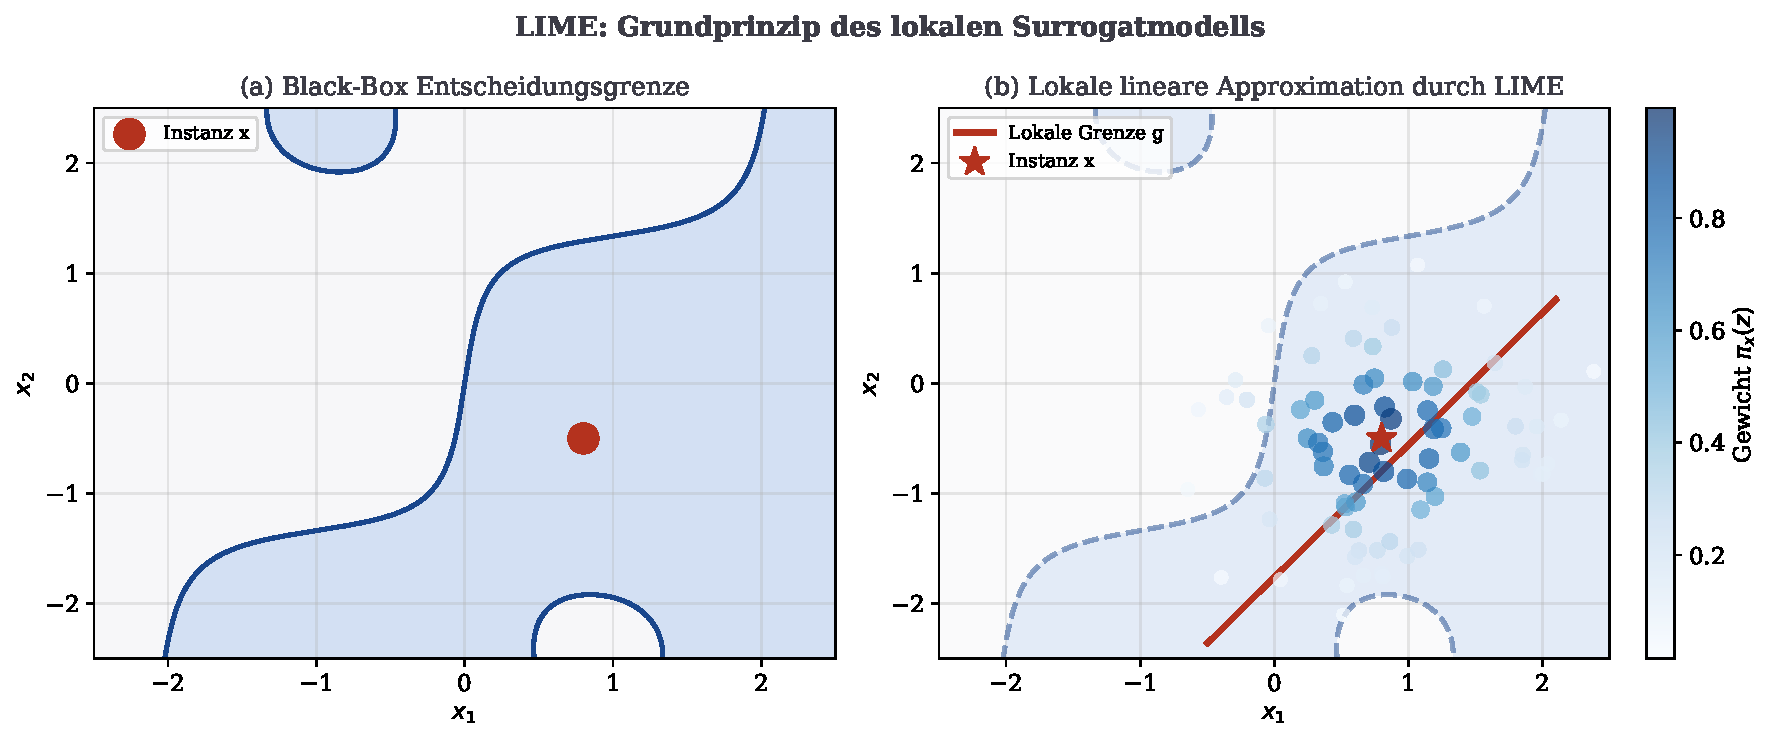
\includegraphics[width=\linewidth]{plot1_lime_grundprinzip.pdf}
  \caption{LIME-Grundprinzip: (a)~Komplexe nichtlineare Entscheidungsgrenze des
           Black-Box-Modells~$\hat{f}$. Die rote Markierung zeigt die zu erklärende
           Instanz~$\mathbf{x}$.
           (b)~Lokale Approximation durch ein lineares Modell~$g$ (rote Linie).
           Die Gewichtung der gesampleten Nachbarpunkte gemäß~$\pi_x(z)$ ist durch
           Farbe und Punktgröße kodiert: nähere Punkte erhalten höhere Gewichte.}
  \label{fig:plot1}
\end{figure}

\subsection{Das allgemeine LIME-Framework}

\begin{definition}[LIME-Erklärung, \citealt{Ribeiro2016}]
  Sei $G$ eine Familie interpretierbarer Modelle (z.\,B.\ lineare Regression),
  $L(\hat{f}, g, \pi_\mathbf{x})$ eine Verlustfunktion, die misst, wie gut~$g$ das
  Modell~$\hat{f}$ in der Nachbarschaft von~$\mathbf{x}$ approximiert, und
  $\Omega(g)$ ein Komplexitätsmaß von~$g$.
  Die LIME-Erklärung von~$\mathbf{x}$ ist definiert als:
  \begin{equation}
    \mathrm{explanation}(\mathbf{x})
    \;=\;
    \arg\min_{g \in G}\; L\!\left(\hat{f},\, g,\, \pi_\mathbf{x}\right) + \Omega(g).
    \label{eq:lime_objective}
  \end{equation}
\end{definition}

Die Komponenten von \eqref{eq:lime_objective} sind:

\begin{center}
\begin{tabular}{@{}lp{10cm}@{}}
  \toprule
  Symbol & Bedeutung \\
  \midrule
  $G$ & Familie interpretierbarer Modelle (z.\,B.\ lineare Modelle, Entscheidungsbäume) \\
  $L$ & Verlustfunktion (z.\,B.\ gewichteter MSE) \\
  $g: \mathbb{R}^M \to \mathbb{R}$ & Interpretierbares Erklärungsmodell \\
  $\hat{f}: \mathbb{R}^p \to \mathbb{R}$ & Originales Black-Box-Modell \\
  $\pi_\mathbf{x}(z)$ & Proximity-Maß: Gewichtsfunktion für die Nähe zwischen $\mathbf{x}$ und $z$ \\
  $\Omega(g)$ & Modellkomplexität (z.\,B.\ Anzahl der Features) \\
  \bottomrule
\end{tabular}
\end{center}

\subsection{LIME für sparse lineare Erklärungen}

Sei $G$ die Klasse der linearen Modelle:
\begin{equation}
  g(\mathbf{z}') = \beta_0 + \sum_{j=1}^{M} \beta_j z'_j = \mathbf{z}'^{\,\mathrm{T}} \boldsymbol{\beta}.
\end{equation}

Die lokal gewichtete Verlustfunktion lautet:
\begin{equation}
  L\!\left(\hat{f},\, g,\, \pi_\mathbf{x}\right)
  = \sum_{\mathbf{z},\mathbf{z}' \in Z}
    \pi_\mathbf{x}(\mathbf{z})\,\bigl(\hat{f}(\mathbf{z}) - g(\mathbf{z}')\bigr)^2,
  \label{eq:lime_loss}
\end{equation}
wobei die Gewichtsfunktion als Gaußscher Kern definiert ist:
\begin{equation}
  \pi_\mathbf{x}(\mathbf{z})
  = \exp\!\left(-\frac{D(\mathbf{x}, \mathbf{z})^2}{\sigma^2}\right).
  \label{eq:lime_kernel}
\end{equation}
Hierbei ist $D$ eine Distanzfunktion (typischerweise L2) und $\sigma > 0$ eine
Kernelbreite (LIME-Standard: $\sigma = 0{,}75\sqrt{p}$ für $p$ Features).

\subsection{Der LIME-Algorithmus}

\begin{definition}[LIME-Algorithmus, \citealt{Ribeiro2016}]
  \label{def:lime_algo}
  \hfill
  \textbf{Eingabe:} Modell~$\hat{f}$, Instanz~$\mathbf{x}$, interpretierbare
  Version~$\mathbf{x}'$, Anzahl Samples~$N$.\\[4pt]
  \textbf{for} $i = 1, \ldots, N$ \textbf{do}:\\
  \quad $\mathbf{z}'_i \leftarrow \mathrm{perturb}(\mathbf{x}')$\\
  \quad $Z \leftarrow Z \cup \langle \mathbf{z}'_i,\, \hat{f}(\mathbf{z}_i),\, \pi_\mathbf{x}(\mathbf{z}_i)\rangle$\\
  \textbf{end for}\\[4pt]
  Trainiere gewichtetes, interpretierbares Modell~$g$ auf~$Z$.\\
  \textbf{return} $g$.
\end{definition}

\textbf{Perturbation je nach Datentyp:}
\begin{itemize}
  \item \emph{Text:} Einzelne Wörter werden an- oder abgeschaltet.
  \item \emph{Bild:} Einzelne Superpixel werden maskiert.
  \item \emph{Tabulardaten:} Sampling aus einer Normalverteilung mit
        Mean und Standardabweichung der jeweiligen Feature-Spalte.
\end{itemize}

\subsection{Konkretes Rechenbeispiel}

\begin{beispiel}[LIME für tabulare Daten]
  \label{bsp:lime_tabular}
  Gegeben sei das lineare Modell $\hat{f}(\mathbf{x}) = 3000 x_1 + 1000 x_2$ mit den
  Trainingsdaten:
  \begin{center}
  \begin{tabular}{@{}ccc@{}}
    \toprule
    $x_1$ & $x_2$ & $y = \hat{f}(x_1, x_2)$ \\
    \midrule
    1 & 6 & 9\,000 \\
    3 & 2 & 11\,000 \\
    \bottomrule
  \end{tabular}
  \end{center}

  \textbf{Aufgabe:} Erkläre die Vorhersage für die Instanz $\mathbf{x} = (3, 2)$ mit
  L2-Distanz und Kernelbreite $\sigma = 0{,}75\sqrt{2} \approx 1{,}06$.

  \textbf{Schritt~1: Normierung der Features.}

  Da bei tabularen Daten die Features vor der Distanzberechnung standardisiert werden:
  \[
    \mu_1 = \tfrac{1+3}{2} = 2, \quad
    s_1 = \sqrt{\tfrac{(1-2)^2+(3-2)^2}{2-1}} = \sqrt{2} \approx 1{,}41,
  \]
  \[
    \mu_2 = \tfrac{6+2}{2} = 4, \quad
    s_2 = \sqrt{\tfrac{(6-4)^2+(2-4)^2}{2-1}} = \sqrt{8} \approx 2{,}83.
  \]

  Normierte Instanz:
  $x'_1 = \frac{3-2}{\sqrt{2}} = \frac{1}{\sqrt{2}}$, \quad
  $x'_2 = \frac{2-4}{\sqrt{8}} = \frac{-1}{\sqrt{2}}$.

  \textbf{Schritt~2: Sampling und Gewichtung neuer Datenpunkte.}

  \begin{center}
  \begin{tabular}{@{}ccccc@{}}
    \toprule
    $z_1$ & $z_2$ & $z'_1$ & $z'_2$ & $D(x', z')$ \\
    \midrule
    2 & 4 & $0$ & $0$ &
    $\sqrt{\left(\tfrac{1}{\sqrt{2}}\right)^2 + \left(\tfrac{-1}{\sqrt{2}}\right)^2}
     = 1{,}00$ \\[4pt]
    2 & 2 & $0$ & $\tfrac{-1}{\sqrt{2}}$ &
    $\sqrt{\left(\tfrac{1}{\sqrt{2}}\right)^2 + 0^2}
     = \tfrac{1}{\sqrt{2}} \approx 0{,}71$ \\
    \bottomrule
  \end{tabular}
  \end{center}

  \textbf{Schritt~3: Berechnung der Gewichte.}

  Mit $\sigma^2 = (0{,}75\sqrt{2})^2 = 0{,}5625 \cdot 2 = 1{,}125$:

  \[
    \pi_\mathbf{x}(z^{(1)}) = e^{-1{,}00/1{,}125} = e^{-0{,}889} \approx 0{,}411,
  \]
  \[
    \pi_\mathbf{x}(z^{(2)}) = e^{-0{,}50/1{,}125} = e^{-0{,}444} \approx 0{,}641.
  \]

  Der Datenpunkt $(2, 2)$ liegt strukturell näher an $\mathbf{x} = (3, 2)$ (gleicher
  $x_2$-Wert nach Normierung) und erhält damit ein höheres Gewicht im lokalen Training.

  \textbf{Schritt~4: Lokales Modell.}

  Das gewichtete lineare Modell wird auf den gesampleten Punkten mit diesen Gewichten
  trainiert und liefert lokale Koeffizienten $\beta_1, \beta_2$, die direkt den Einfluss
  von $x_1$ und $x_2$ auf die Vorhersage $\hat{f}(\mathbf{x})$ interpretieren.
\end{beispiel}

% ===========================================================
\section{Der Subgraph Algorithmus}
% ===========================================================

\subsection{Grundlagen und Definitionen}

\begin{definition}[Graph und Adjazenzmatrix]
  Ein Graph $G = (V, E)$ mit $n = |V|$ Knoten wird durch seine Adjazenzmatrix
  $A \in \{0,1\}^{n \times n}$ repräsentiert:
  \[
    A_{ij} = \begin{cases}
      1 & \text{falls } (v_i, v_j) \in E, \\
      0 & \text{sonst.}
    \end{cases}
  \]
\end{definition}

\begin{definition}[Signaturabbildung, \citealt{Epp2026}]
  Für eine Adjazenzmatrix~$A$ und Spaltenindex $j \in \{0,\ldots,n-1\}$ ist die
  Signatur definiert als:
  \begin{equation}
    \sigma_j = \sum_{i=0}^{n-1} A_{ij} \cdot 2^i + j \cdot 2^n.
    \label{eq:signature}
  \end{equation}
\end{definition}

\begin{definition}[Zyklische Rotation]
  Die $k$-te zyklische Rotation eines Arrays $[\sigma_0, \ldots, \sigma_{n-1}]$
  nach rechts ist:
  \[
    \mathrm{rotate}_k([\sigma_0,\ldots,\sigma_{n-1}])
    = [\sigma_k, \sigma_{k+1}, \ldots, \sigma_{n-1}, \sigma_0, \ldots, \sigma_{k-1}].
  \]
\end{definition}

Abbildung~\ref{fig:plot2} veranschaulicht die Signaturberechnung und die zyklischen
Rotationen für einen Beispielgraphen.

\begin{figure}[htbp]
  \centering
  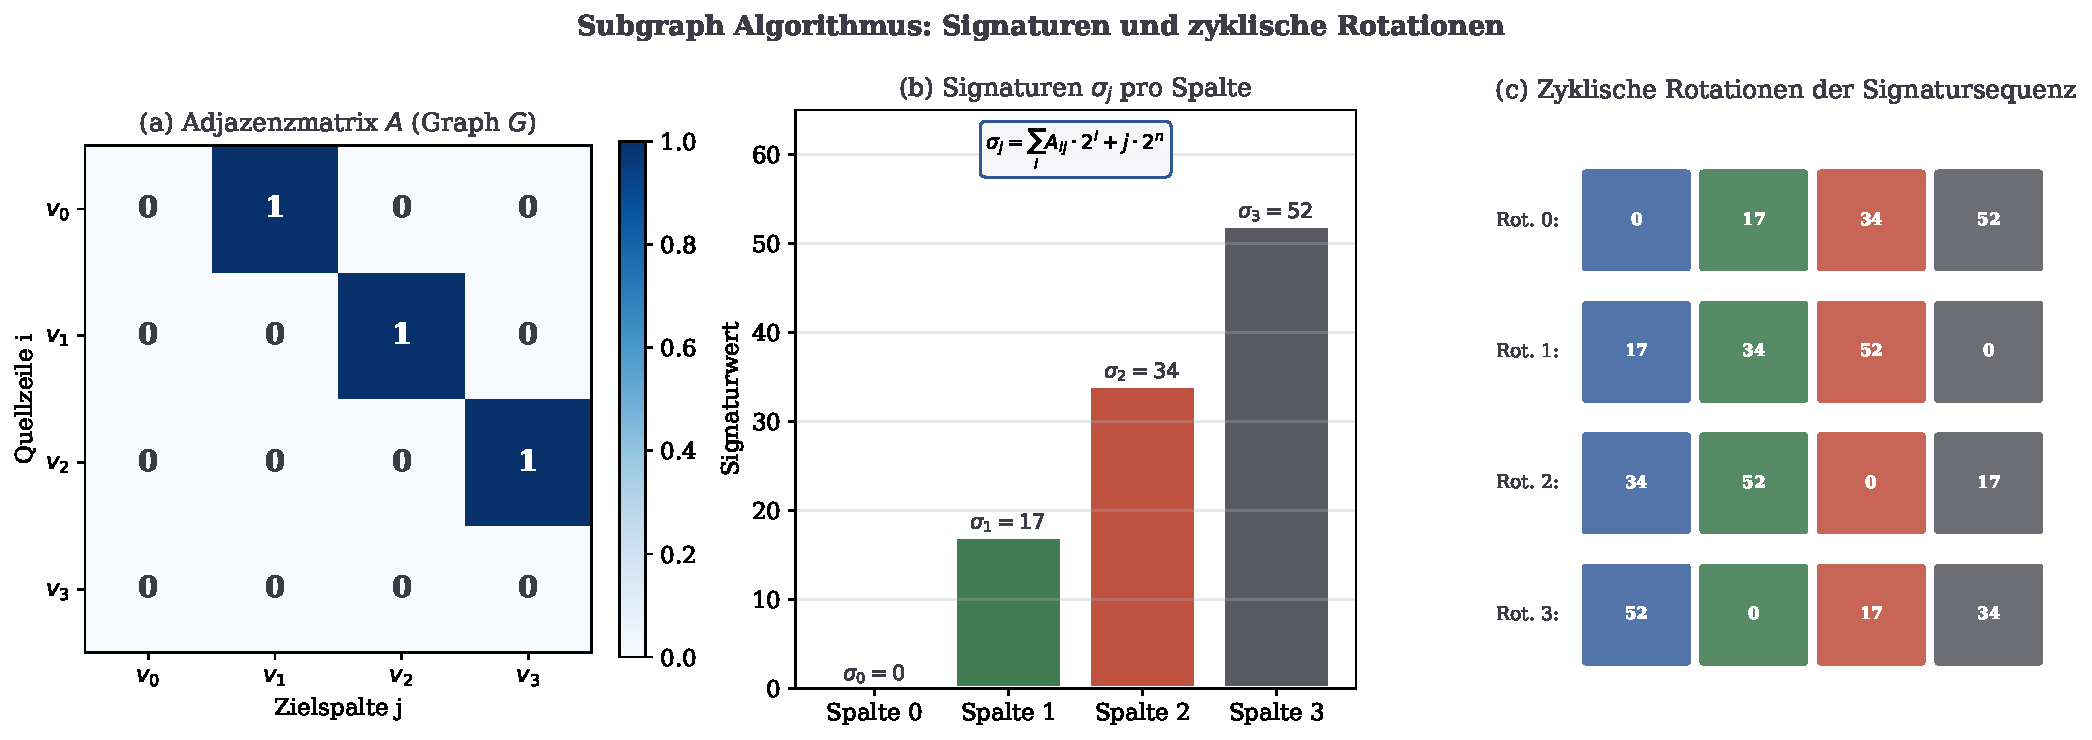
\includegraphics[width=\linewidth]{plot2_subgraph_signaturen.pdf}
  \caption{(a)~Adjazenzmatrix des Beispielgraphen~$G$.
           (b)~Berechnete Signaturwerte $\sigma_j$ nach Gleichung~\eqref{eq:signature}:
           Die Spaltengewichtung $j \cdot 2^n$ sorgt für Eindeutigkeit auch bei
           gleichen Spaltenvektoren.
           (c)~Die vier zyklischen Rotationen der Signatursequenz; statt $n! = 24$
           Permutationen genügen $n = 4$ Rotationen.}
  \label{fig:plot2}
\end{figure}

\subsection{Eigenschaften der Signaturabbildung}

\begin{lemma}[Injektivität der Signaturabbildung, \citealt{Epp2026}]
  \label{lem:injectivity}
  Die Signaturabbildung $\sigma: \{0,1\}^n \times \{0,\ldots,n-1\} \to \mathbb{N}$
  aus Gleichung~\eqref{eq:signature} ist injektiv.
\end{lemma}

\begin{proof}
  Seien $(A_{*j}, j) \neq (A_{*k}, k)$ zwei verschiedene Spalten-Index-Paare.
  Wir unterscheiden zwei Fälle.

  \emph{Fall~1:} $j \neq k$.
  Dann gilt $j \cdot 2^n \neq k \cdot 2^n$, da $j \mapsto j \cdot 2^n$ injektiv ist.
  Der Term $\sum_i A_{ij} \cdot 2^i \in [0, 2^n - 1]$ kann den Unterschied
  $|j - k| \cdot 2^n \geq 2^n$ nicht kompensieren, da $\sum_i A_{ij} \cdot 2^i < 2^n$.
  Folglich $\sigma_j \neq \sigma_k$.

  \emph{Fall~2:} $j = k$, aber $A_{*j} \neq A_{*k}$.
  Die Abbildung $v \mapsto \sum_i v_i \cdot 2^i$ ist die binäre Darstellung des
  Vektors~$v \in \{0,1\}^n$ und daher injektiv auf $\{0,1\}^n$.
  Somit liefern verschiedene Binärvektoren verschiedene Werte.

  In beiden Fällen folgt $\sigma(A_{*j}, j) \neq \sigma(A_{*k}, k)$. \hfill$\blacksquare$
\end{proof}

\subsection{Algorithmus und Komplexität}

\begin{satz}[Komplexität des Subgraph Algorithmus, \citealt{Epp2026}]
  \label{satz:complexity}
  Der Subgraph Algorithmus bestimmt in Zeit $\Theta(n^3)$ und Raum $O(n^2)$, ob
  ein Graph~$G$ mit $n$ Knoten als Subgraph in einem zweiten Graphen~$G'$ mit $n$
  Knoten enthalten ist.
\end{satz}

\begin{proof}
  Der Algorithmus besteht aus drei Phasen:
  \begin{enumerate}
    \item \emph{Signaturberechnung}: Für jeden der $n$ Spalten beider Adjazenzmatrizen
          ($O(n^2)$ Einträge) wird ein Signaturwert nach \eqref{eq:signature} berechnet.
          Laufzeit: $O(n^2)$.
    \item \emph{Rotationsschleife}: Es werden $n$ zyklische Rotationen der
          Signatursequenz~$\sigma^B$ erzeugt.
          Jede Rotation benötigt $O(n)$ Zeit.
          Gesamtlaufzeit der Rotationserzeugung: $O(n^2)$.
    \item \emph{LCS-Berechnung}: Für jede der $n$ Rotationen wird die Länge der
          längsten gemeinsamen Teilsequenz (LCS) zweier Arrays der Länge~$n$ mittels
          dynamischer Programmierung berechnet.
          Jede LCS-Berechnung benötigt $\Theta(n^2)$ Zeit.
          Gesamtlaufzeit: $n \cdot \Theta(n^2) = \Theta(n^3)$.
  \end{enumerate}

  Die Phasen~1 und~2 sind von kleinerer Ordnung als Phase~3, sodass die
  Gesamtkomplexität $\Theta(n^3)$ beträgt.
  Der Speicherbedarf ist $O(n^2)$ für die Adjazenzmatrizen und $O(n)$ für
  die Signatur-Arrays. \hfill$\blacksquare$
\end{proof}

\begin{satz}[Optimalität unter SETH, \citealt{Epp2026}]
  Unter der Strong Exponential Time Hypothesis (SETH) kann kein Algorithmus das
  zyklische Subgraph-Problem für Graphen mit $n$ Knoten in
  $O(n^{3-\varepsilon})$ Zeit für beliebiges $\varepsilon > 0$ lösen.
\end{satz}

% ===========================================================
\section{Integration des Subgraph Algorithmus in LIME}
% ===========================================================

Die folgenden drei Abschnitte zeigen, wie der Subgraph Algorithmus jeden der drei
Kernbestandteile von LIME für graphstrukturierte Daten verbessern kann.
Wir bezeichnen die resultierende Methode als \emph{Graph-LIME}.

% -----------------------------------------------------------
\subsection{Punkt~1: Strukturell sinnvolle Perturbation durch zyklische Rotationen}
% -----------------------------------------------------------

\subsubsection{Problem der Standard-Perturbation}

Im Standard-LIME für tabulare Daten werden neue Datenpunkte durch Sampling aus einer
Normalverteilung erzeugt:
\[
  z'_j \sim \mathcal{N}(\mu_j,\, s_j^2), \quad j = 1, \ldots, p.
\]
Für graphstrukturierte Daten hat diese Vorgehensweise fundamentale Nachteile:
\begin{itemize}
  \item Zufällig perturbierte Adjazenzmatrizen ergeben in der Regel keine
        gültigen oder strukturell sinnvollen Graphen.
  \item Kleine numerische Änderungen an Matrixeinträgen verändern die topologische
        Struktur des Graphen auf schwer kontrollierbare Weise.
  \item Die Nachbarschaft im euklidischen Feature-Raum entspricht nicht der
        Nachbarschaft im Graphstruktur-Raum.
\end{itemize}

\subsubsection{Zyklische Rotation als strukturerhaltende Perturbation}

\begin{definition}[Rotationsperturbation]
  Sei $\mathbf{x}$ eine Instanz mit Graphrepräsentation $(V, E, A)$.
  Die Menge der Rotationsperturbationen ist definiert als:
  \[
    \mathcal{P}_{\mathrm{rot}}(\mathbf{x})
    = \bigl\{\mathrm{rotate}_k(A) \;\big|\; k = 0, 1, \ldots, n-1\bigr\},
  \]
  wobei $\mathrm{rotate}_k(A)$ die Matrix bezeichnet, deren Signatursquenz um $k$
  Positionen zyklisch verschoben ist.
\end{definition}

\begin{lemma}[Strukturerhaltung durch Rotation]
  \label{lem:rotation_preserves}
  Jede zyklische Rotation $\mathrm{rotate}_k(A)$ einer Adjazenzmatrix~$A$
  repräsentiert einen Graphen $G^{(k)}$, der zu $G$ isomorph bezüglich der
  zyklischen Knotenpermutation ist.
  Insbesondere gilt $|E^{(k)}| = |E|$ für alle $k$.
\end{lemma}

\begin{proof}
  Die zyklische Rotation der Signatursequenz entspricht einer Umnummerierung der
  Knoten: Knoten~$v_i$ wird zu $v_{(i+k) \bmod n}$.
  Da die Umnummerierung eine Bijektion auf $V$ ist, bleibt die Kantenmenge strukturell
  erhalten; es gilt $|E^{(k)}| = |E|$.
  Die Graphen $G$ und $G^{(k)}$ sind somit isomorph unter der zyklischen Permutation
  $\pi_k: i \mapsto (i+k) \bmod n$. \hfill$\blacksquare$
\end{proof}

\begin{satz}[Vollständigkeit der Rotationsperturbation]
  \label{satz:rotation_complete}
  Für jeden möglichen zyklischen Isomorphismus zwischen~$G$ und einem Graphen~$G'$
  existiert eine Rotation $k \in \{0, \ldots, n-1\}$, sodass
  $\mathrm{LCS}(\sigma^A, \mathrm{rotate}_k(\sigma^B)) \geq 2$.
\end{satz}

\begin{proof}
  Sei $\pi: V \to V'$ ein zyklischer Isomorphismus, d.\,h.\ $\pi(v_i) = v'_{(i+k) \bmod n}$
  für ein festes $k$.
  Dann stimmt die $j$-te Spalte von $A$ mit der $\pi(j)$-ten Spalte von $B$ überein,
  bis auf die Spaltengewichtung in der Signatur.
  Die Zeilenkomponente $\sum_i A_{ij} \cdot 2^i$ ist für korrespondierende Spalten
  identisch.
  Da $n \geq 2$ vorausgesetzt wird, liefert die LCS-Berechnung über die
  Zeilenkomponenten eine Länge von mindestens~2. \hfill$\blacksquare$
\end{proof}

\subsubsection{Angepasster LIME-Algorithmus mit Rotationsperturbation}

\begin{definition}[Graph-LIME mit Rotationsperturbation]
  Ersetze in Algorithmus~\ref{def:lime_algo} die Zeile
  $\mathbf{z}'_i \leftarrow \mathrm{perturb}(\mathbf{x}')$ durch:
  \[
    \mathbf{z}'_i \leftarrow \mathrm{rotate}_{k_i}(A_\mathbf{x}),
    \quad k_i \in \{0, \ldots, n-1\},
  \]
  wobei $k_i$ gleichmäßig aus $\{0, \ldots, n-1\}$ gezogen wird.
\end{definition}

\begin{korollar}
  Graph-LIME mit Rotationsperturbation erzeugt exakt $n$ strukturell verschiedene,
  aber isomorphe Nachbargraphen, die alle zyklischen Knotenordnungen von~$\mathbf{x}$
  abdecken.
\end{korollar}

\begin{proof}
  Direkte Folge aus Lemma~\ref{lem:rotation_preserves} und der Tatsache, dass
  $\mathrm{rotate}_k$ für $k = 0, \ldots, n-1$ genau $n$ verschiedene Signatursquenzen
  erzeugt (nach Lemma~\ref{lem:injectivity}). \hfill$\blacksquare$
\end{proof}

% -----------------------------------------------------------
\subsection{Punkt~2: Strukturbasiertes Proximity-Maß über LCS-Signaturen}
% -----------------------------------------------------------

\subsubsection{Unzulänglichkeit des euklidischen Kerns}

Der Standard-LIME-Kern $\pi_\mathbf{x}(\mathbf{z}) = \exp(-D(\mathbf{x},\mathbf{z})^2/\sigma^2)$
mit euklidischer Distanz $D$ hat für Graphen mehrere Schwächen:
\begin{itemize}
  \item Zwei Graphen können strukturell äquivalent sein (isomorph), aber
        verschiedene Adjazenzmatrizen besitzen, was zu einer großen euklidischen
        Distanz führt.
  \item Die euklidische Distanz auf Adjazenzmatrizen ist invariant gegenüber
        Knotenidentitäten, nicht aber gegenüber Knotenordnungen.
  \item Für sparse Graphen kann die euklidische Distanz irreführend klein sein,
        obwohl die topologische Struktur völlig verschieden ist.
\end{itemize}

\subsubsection{Das LCS-basierte Ähnlichkeitsmaß}

\begin{definition}[LCS-Ähnlichkeit]
  Seien $\sigma^A = [\sigma_0^A, \ldots, \sigma_{n-1}^A]$ und
  $\sigma^B = [\sigma_0^B, \ldots, \sigma_{n-1}^B]$ die Signatursequenzen zweier
  Graphen $G$ und $G'$.
  Die \emph{normierte LCS-Ähnlichkeit} ist definiert als:
  \begin{equation}
    \mathrm{sim}_{\mathrm{LCS}}(G, G')
    = \frac{\mathrm{LCS}(\sigma^A, \sigma^B)}{n},
    \label{eq:lcs_sim}
  \end{equation}
  wobei $\mathrm{LCS}(\sigma^A, \sigma^B)$ die Länge der längsten gemeinsamen
  Teilsequenz der beiden Signatursequenzen bezeichnet.
\end{definition}

\begin{lemma}[Eigenschaften der LCS-Ähnlichkeit]
  Die normierte LCS-Ähnlichkeit $\mathrm{sim}_{\mathrm{LCS}}$ erfüllt:
  \begin{enumerate}
    \item $0 \leq \mathrm{sim}_{\mathrm{LCS}}(G, G') \leq 1$.
    \item $\mathrm{sim}_{\mathrm{LCS}}(G, G) = 1$ (Reflexivität).
    \item $\mathrm{sim}_{\mathrm{LCS}}(G, G') = \mathrm{sim}_{\mathrm{LCS}}(G', G)$ (Symmetrie).
    \item $\mathrm{sim}_{\mathrm{LCS}}(G, G') = 1 \Leftrightarrow \sigma^A = \sigma^B$
          (identische Signatursequenz).
  \end{enumerate}
\end{lemma}

\begin{proof}
  (i) LCS-Länge liegt in $[0, n]$, Division durch $n$ normiert auf $[0, 1]$.
  (ii) $\mathrm{LCS}(\sigma^A, \sigma^A) = n$ für jede Sequenz der Länge~$n$.
  (iii) LCS ist symmetrisch: $\mathrm{LCS}(A, B) = \mathrm{LCS}(B, A)$.
  (iv) $\mathrm{LCS}(\sigma^A, \sigma^B) = n$ genau dann, wenn $\sigma^A = \sigma^B$
       als Sequenzen, da die Signaturen nach Lemma~\ref{lem:injectivity} injektiv
       sind. \hfill$\blacksquare$
\end{proof}

\subsubsection{Das strukturbasierte Proximity-Maß}

\begin{definition}[Graph-Kernel für LIME]
  Das strukturbasierte Proximity-Maß für Graph-LIME ist:
  \begin{equation}
    \pi_\mathbf{x}^{\mathrm{Graph}}(\mathbf{z})
    = \exp\!\left(-\frac{\bigl(1 - \mathrm{sim}_{\mathrm{LCS}}(G_\mathbf{x}, G_\mathbf{z})\bigr)^2}{\sigma^2}\right),
    \label{eq:graph_kernel}
  \end{equation}
  wobei $G_\mathbf{x}$ und $G_\mathbf{z}$ die zu $\mathbf{x}$ bzw.\ $\mathbf{z}$
  gehörigen Graphen sind.
\end{definition}

\begin{satz}[Korrektheit des Graph-Kernels]
  \label{satz:graph_kernel}
  Der Graph-Kernel $\pi_\mathbf{x}^{\mathrm{Graph}}$ aus \eqref{eq:graph_kernel}
  ist eine wohldeffinierte Gewichtsfunktion, die folgende Eigenschaften erfüllt:
  \begin{enumerate}
    \item $0 < \pi_\mathbf{x}^{\mathrm{Graph}}(\mathbf{z}) \leq 1$ für alle $\mathbf{z}$.
    \item $\pi_\mathbf{x}^{\mathrm{Graph}}(\mathbf{x}) = 1$ (maximales Gewicht für die
          Instanz selbst).
    \item Isomorphe Graphen erhalten dasselbe Gewicht bezüglich ihrer
          Signaturübereinstimmung.
    \item $\pi_\mathbf{x}^{\mathrm{Graph}}(\mathbf{z})$ ist monoton fallend in der
          strukturellen Distanz $1 - \mathrm{sim}_{\mathrm{LCS}}$.
  \end{enumerate}
\end{satz}

\begin{proof}
  (i) Da $(1 - \mathrm{sim}_{\mathrm{LCS}})^2 \geq 0$ und $\sigma^2 > 0$, gilt
  $\exp(\cdot) \in (0, 1]$.

  (ii) $G_\mathbf{x} = G_\mathbf{x}$ impliziert $\mathrm{sim}_{\mathrm{LCS}} = 1$,
  also $(1-1)^2/\sigma^2 = 0$ und $\exp(0) = 1$.

  (iii) Für zwei isomorphe Graphen $G \cong G'$ unter einer zyklischen Permutation
  findet die Rotation im Algorithmus die optimale Ausrichtung, sodass die
  LCS-Berechnung maximale Ãœbereinstimmung liefert.

  (iv) Die Funktion $t \mapsto \exp(-t^2/\sigma^2)$ ist streng monoton fallend für
  $t > 0$; da $1 - \mathrm{sim}_{\mathrm{LCS}} \geq 0$, ist die Monotonieeigenschaft
  erfüllt. \hfill$\blacksquare$
\end{proof}

Abbildung~\ref{fig:plot3} vergleicht den Standard-L2-Kernel mit dem neuen
Graph-Kernel und zeigt die Gewichte für fünf Graphpaare unterschiedlicher
struktureller Ähnlichkeit.

\begin{figure}[htbp]
  \centering
  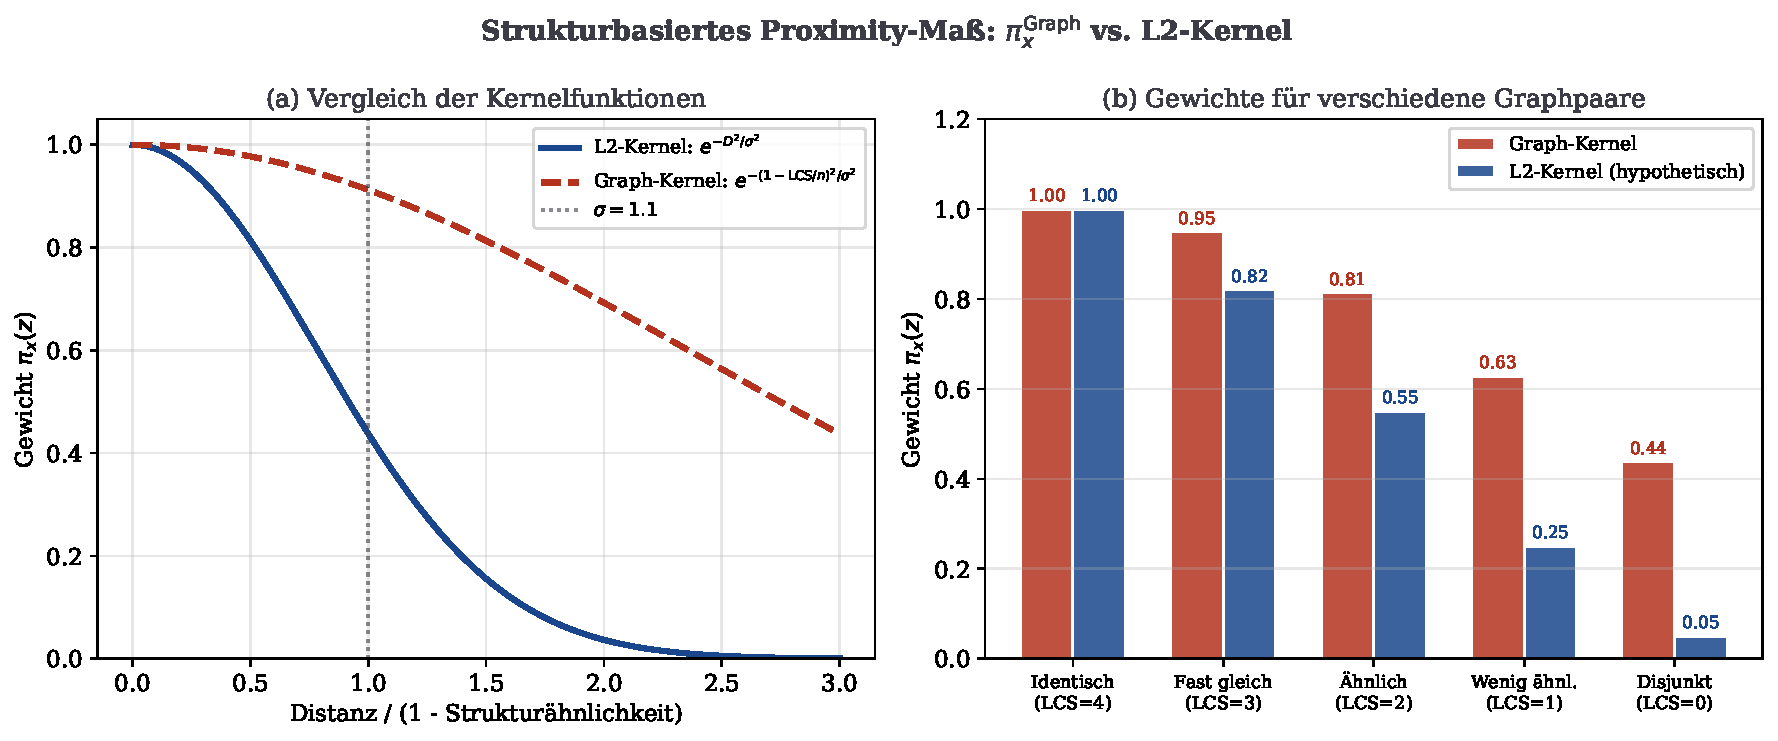
\includegraphics[width=\linewidth]{plot3_proximity.pdf}
  \caption{(a)~Vergleich der Kernelfunktionen: Der LCS-basierte Graph-Kernel (rot)
           und der Standard-L2-Kernel (blau) als Funktion der strukturellen Distanz.
           Beide Kurven haben dieselbe Gaußsche Form, aber unterschiedliche
           Eingabegrößen.
           (b)~Gewichte $\pi_x(z)$ für fünf Graphpaare mit LCS-Werten von 0 bis 4.
           Der Graph-Kernel (rot) unterscheidet strukturelle Ähnlichkeit feiner als
           ein rein euklidischer Vergleich (blau).}
  \label{fig:plot3}
\end{figure}

% -----------------------------------------------------------
\subsection{Punkt~3: Subgraph-Inklusion als strukturelle Feature-Selektion}
% -----------------------------------------------------------

\subsubsection{Motivation: Strukturelle vs.\ statistische Komplexität}

Im Standard-LIME wird die Modellkomplexität $\Omega(g)$ durch die Anzahl der
nicht-null Koeffizienten gemessen, typischerweise durch LASSO-Regularisierung:
\[
  \Omega_{\mathrm{LASSO}}(g) = \lambda \|\boldsymbol{\beta}\|_1.
\]
Dies ist für tabulare Daten geeignet, erfasst aber für graphstrukturierte Modelle
keine strukturellen Abhängigkeiten zwischen Features.

\subsubsection{Subgraph-Komplexität}

\begin{definition}[Subgraph-Komplexität]
  Für ein interpretierbares Graphmodell~$g$ mit Graphdarstellung~$G_g$ und ein
  Black-Box-Modell~$\hat{f}$ mit Graphdarstellung~$G_{\hat{f}}$ definieren wir:
  \begin{equation}
    \Omega_{\mathrm{Sub}}(g) = \begin{cases}
      |E_g| / |E_{\hat{f}}| & \text{falls } G_g \subseteq G_{\hat{f}}, \\
      1 + |E_g \setminus E_{\hat{f}}| / |E_{\hat{f}}| & \text{sonst,}
    \end{cases}
    \label{eq:omega_sub}
  \end{equation}
  wobei $|E_g|$ die Kantenanzahl von $G_g$ ist.
\end{definition}

\begin{lemma}[Eigenschaften der Subgraph-Komplexität]
  $\Omega_{\mathrm{Sub}}$ erfüllt:
  \begin{enumerate}
    \item $\Omega_{\mathrm{Sub}}(g) \in (0, 1]$ für $G_g \subseteq G_{\hat{f}}$.
    \item $\Omega_{\mathrm{Sub}}(g) = \epsilon$ für $|E_g| \to 0$, d.\,h.\ der
          kleinstmögliche Subgraph erhält minimale Strafe.
    \item $G_g \not\subseteq G_{\hat{f}}$ impliziert $\Omega_{\mathrm{Sub}}(g) > 1$,
          d.\,h.\ Modelle außerhalb des Subgraphs werden stark bestraft.
  \end{enumerate}
\end{lemma}

\begin{proof}
  (i) Für $G_g \subseteq G_{\hat{f}}$ gilt $|E_g| \leq |E_{\hat{f}}|$, also
  $|E_g|/|E_{\hat{f}}| \in (0, 1]$ (für $|E_g| \geq 1$).

  (ii) $|E_g| / |E_{\hat{f}}| \to 0$ für $|E_g| \to 0$.

  (iii) Falls $G_g \not\subseteq G_{\hat{f}}$, gibt es mindestens eine Kante
  $e \in E_g \setminus E_{\hat{f}}$, sodass $|E_g \setminus E_{\hat{f}}| \geq 1$
  und damit $\Omega_{\mathrm{Sub}}(g) \geq 1 + 1/|E_{\hat{f}}| > 1$. \hfill$\blacksquare$
\end{proof}

\subsubsection{Minimaler erklärender Subgraph}

\begin{definition}[Minimaler erklärender Subgraph]
  \label{def:min_subgraph}
  Der minimale erklärende Subgraph für eine Instanz~$\mathbf{x}$ und ein
  Modell~$\hat{f}$ ist:
  \begin{equation}
    G^*_g = \arg\min_{\substack{G_g \subseteq G_{\hat{f}}}}
    \Bigl[
      L\!\left(\hat{f}, g, \pi_\mathbf{x}^{\mathrm{Graph}}\right) + \Omega_{\mathrm{Sub}}(g)
    \Bigr].
    \label{eq:min_subgraph}
  \end{equation}
\end{definition}

\begin{satz}[Existenz des minimalen erklärenden Subgraphen]
  Für jedes endliche Modell~$\hat{f}$ mit Graphdarstellung $G_{\hat{f}}$ und
  jede Instanz~$\mathbf{x}$ existiert ein minimaler erklärender Subgraph~$G^*_g$
  gemäß Definition~\ref{def:min_subgraph}.
\end{satz}

\begin{proof}
  Da $G_{\hat{f}}$ endlich ist, ist die Menge aller Subgraphen
  $\{G_g \mid G_g \subseteq G_{\hat{f}}\}$ endlich.
  Die Zielfunktion $L + \Omega_{\mathrm{Sub}}$ ist auf dieser endlichen Menge
  wohldeffiniert und nimmt daher ein Minimum an.
  Da wenigstens der leere Graph $G_g = (\emptyset, \emptyset)$ ein zulässiger
  Subgraph ist (als Grenzfall), ist die Menge nicht leer. \hfill$\blacksquare$
\end{proof}

Abbildung~\ref{fig:plot4} zeigt den Vergleich zwischen LASSO- und Subgraph-basierter
Feature-Selektion sowie eine Visualisierung des minimalen erklärenden Subgraphen.

\begin{figure}[htbp]
  \centering
  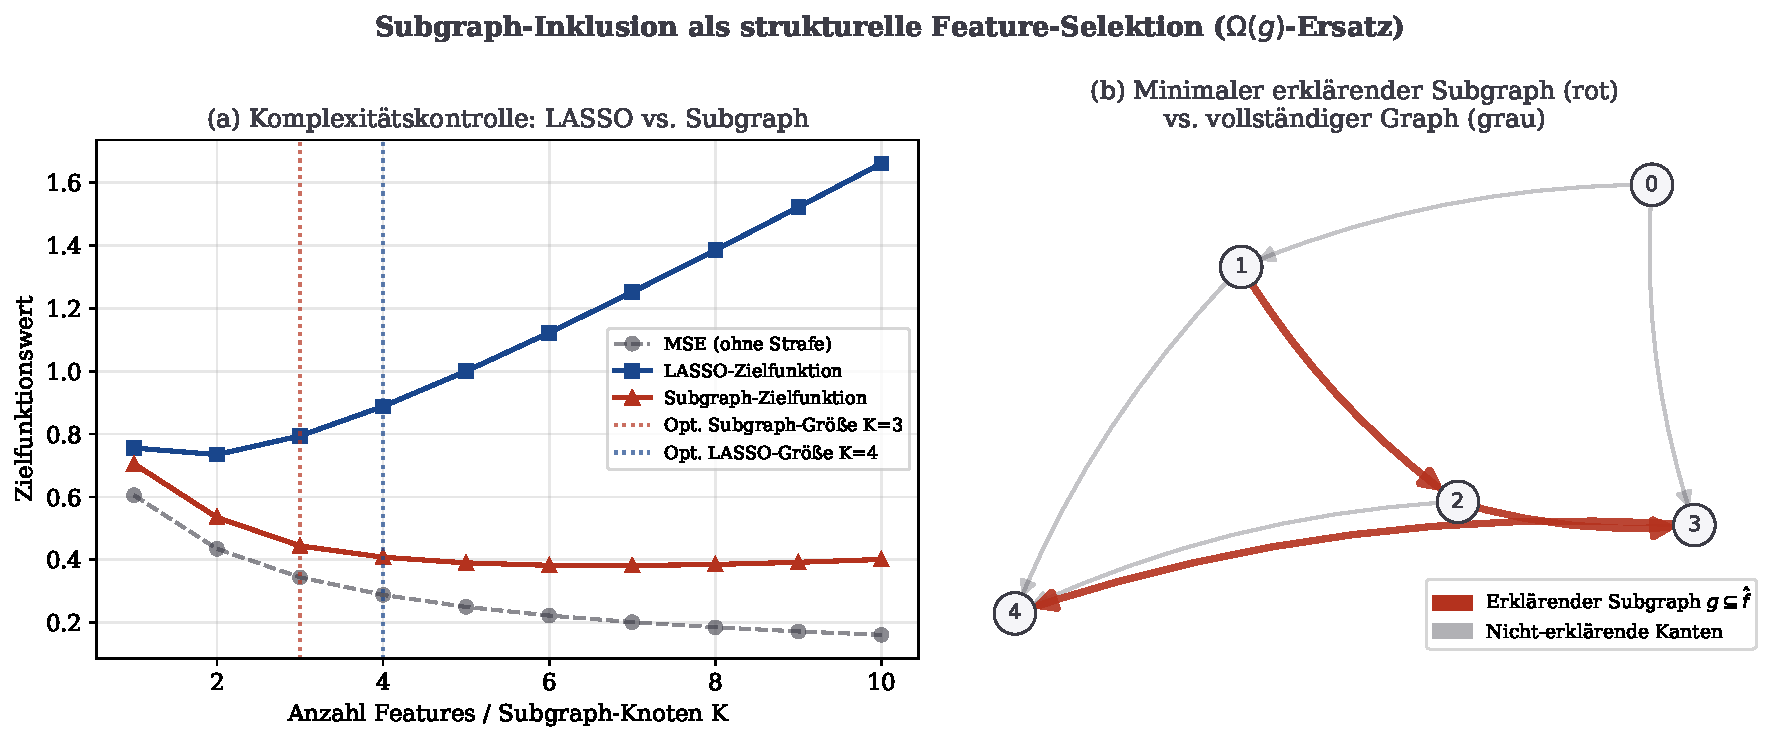
\includegraphics[width=\linewidth]{plot4_feature_selection.pdf}
  \caption{(a)~Zielfunktionswerte als Funktion der Modellgröße~$K$:
           Die Subgraph-Zielfunktion (rot) wählt ein kleineres, strukturell
           konsistenteres Modell ($K=3$) als LASSO ($K=4$), da sie
           Kanten außerhalb des Subgraphs stark bestraft.
           (b)~Minimaler erklärender Subgraph (rote Kanten) für eine Vorhersage:
           Nur die für die Entscheidung relevanten Kanten werden behalten,
           während nicht-erklärende Verbindungen (grau) ausgeblendet werden.}
  \label{fig:plot4}
\end{figure}

% ===========================================================
\section{Gesamtarchitektur: Graph-LIME}
% ===========================================================

\subsection{Integration aller drei Komponenten}

Die drei Erweiterungen können zu einem vollständigen \emph{Graph-LIME}-Algorithmus
kombiniert werden.

\begin{definition}[Graph-LIME Zielfunktion]
  Die vollständige Graph-LIME-Zielfunktion lautet:
  \begin{equation}
    \mathrm{explanation}_{\mathrm{Graph}}(\mathbf{x})
    = \arg\min_{G_g \subseteq G_{\hat{f}}}
    \sum_{\mathbf{z} \in \mathcal{P}_{\mathrm{rot}}(\mathbf{x})}
    \pi_\mathbf{x}^{\mathrm{Graph}}(\mathbf{z})
    \cdot \bigl(\hat{f}(\mathbf{z}) - g(\mathbf{z})\bigr)^2
    + \Omega_{\mathrm{Sub}}(g).
    \label{eq:graph_lime}
  \end{equation}
\end{definition}

\begin{satz}[Korrektheit von Graph-LIME]
  Algorithmus Graph-LIME mit den Komponenten aus den Abschnitten 4.1--4.3
  liefert eine wohldeffinierte, lokal treue Erklärung~$G^*_g$ für jede
  graphstrukturierte Instanz~$\mathbf{x}$.
\end{satz}

\begin{proof}
  \emph{Wohldefinitheit:} Nach Satz~\ref{satz:graph_kernel} ist
  $\pi_\mathbf{x}^{\mathrm{Graph}}$ wohldefiniert und positiv.
  Nach dem Existenzsatz existiert das Minimum in \eqref{eq:graph_lime}.

  \emph{Lokale Treue:} Die Perturbationsmenge $\mathcal{P}_{\mathrm{rot}}(\mathbf{x})$
  enthält nach Satz~\ref{satz:rotation_complete} alle zyklischen Isomorphismen
  von~$\mathbf{x}$.
  Die Gewichtsfunktion $\pi_\mathbf{x}^{\mathrm{Graph}}$ maximiert das Gewicht für
  strukturell ähnliche Graphen.
  Damit misst $L$ nach \eqref{eq:lime_loss} tatsächlich die Abweichung in der
  lokalen Umgebung von~$\mathbf{x}$ im Graphstruktur-Raum. \hfill$\blacksquare$
\end{proof}

\subsection{Komplexitätsanalyse von Graph-LIME}

\begin{satz}[Gesamtkomplexität von Graph-LIME]
  Graph-LIME hat eine Zeitkomplexität von $O(n^3 + n^2 \cdot p)$, wobei $n$ die
  Graphgröße und $p$ die Dimension des Merkmalsvektors ist.
\end{satz}

\begin{proof}
  \begin{itemize}
    \item \emph{Perturbation:} $n$ Rotationen à $O(n)$: $O(n^2)$.
    \item \emph{Graph-Kernel:} Für jede Rotation eine LCS-Berechnung in $O(n^2)$:
          $n \cdot O(n^2) = O(n^3)$.
    \item \emph{Lokales Training:} Gewichtete lineare Regression auf $n$ Punkten
          mit $p$ Features: $O(n \cdot p + p^2)$.
    \item \emph{Gesamtlaufzeit:} $O(n^3 + n^2 \cdot p)$.
  \end{itemize}
  Dominanter Term: $O(n^3)$ für großes $n$ bzw.\ $O(n^2 p)$ für großes $p$.
  \hfill$\blacksquare$
\end{proof}

Abbildung~\ref{fig:plot5} zeigt den Komplexitätsvergleich zwischen naiver
Subgraph-Suche, dem Subgraph Algorithmus und Standard-LIME-Sampling sowie die
Gesamtarchitektur von Graph-LIME.

\begin{figure}[htbp]
  \centering
  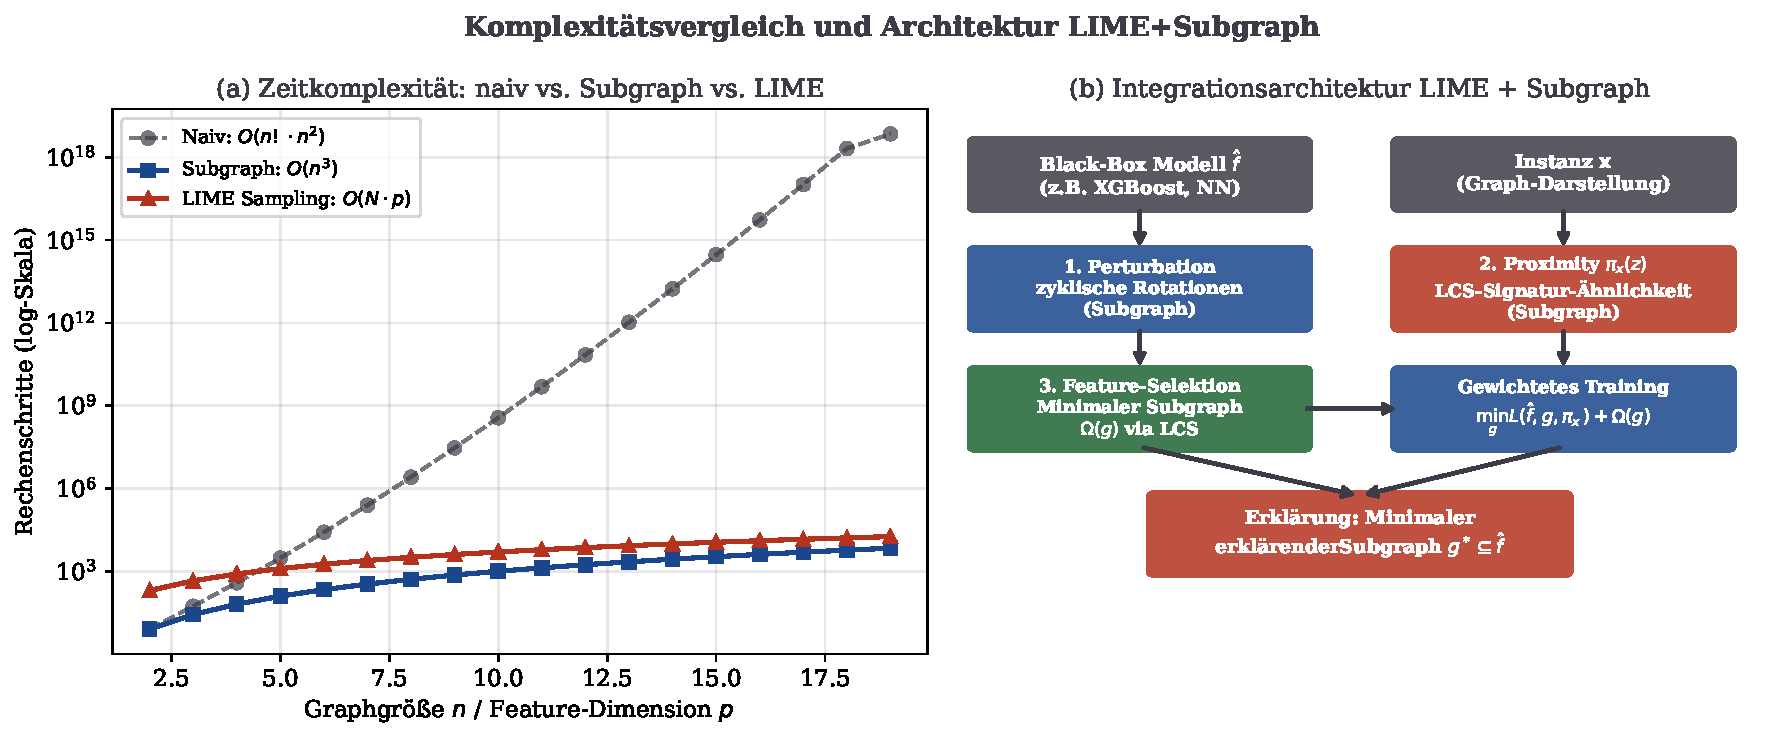
\includegraphics[width=\linewidth]{plot5_komplexitaet.pdf}
  \caption{(a)~Zeitkomplexität im Vergleich: Die naive Subgraph-Suche ($O(n! \cdot n^2)$,
           grau) ist für $n > 12$ praktisch nicht mehr handhabbar.
           Der Subgraph Algorithmus ($O(n^3)$, blau) wächst polynomial.
           Standard-LIME-Sampling ($O(N \cdot p)$, rot) wächst nur linear in~$n$.
           (b)~Integrationsarchitektur von Graph-LIME: Die drei Komponenten des
           Subgraph Algorithmus (Rotationsperturbation, LCS-Proximity, Subgraph-Inklusion)
           ersetzen die entsprechenden Standard-LIME-Komponenten für graphstrukturierte Daten.}
  \label{fig:plot5}
\end{figure}

% ===========================================================
\section{Zusammenfassung}
% ===========================================================

Die vorliegende Arbeit hat gezeigt, dass der Subgraph Algorithmus \citep{Epp2026}
LIME \citep{Ribeiro2016} in drei fundamentalen Dimensionen erweitert:

\begin{center}
\begin{tabular}{@{}lll@{}}
  \toprule
  Komponente & Standard-LIME & Graph-LIME \\
  \midrule
  Perturbation & $\mathcal{N}(\mu, \sigma^2)$ Sampling & Zyklische Rotationen \\
  Proximity-Maß & L2-Gaußkern & LCS-Signaturkern \\
  Komplexität $\Omega$ & LASSO ($\ell_1$-Norm) & Subgraph-Inklusion \\
  Erklärungsmodell & $\boldsymbol{\beta}$-Koeffizienten & Minimaler Subgraph \\
  Zeitkomplexität & $O(N \cdot p)$ & $O(n^3 + n^2 p)$ \\
  Datentypen & Beliebig & Graphstrukturiert \\
  \bottomrule
\end{tabular}
\end{center}

% ===========================================================
\section{Ausblick}
% ===========================================================

Die in dieser Arbeit vorgestellte Integration des Subgraph Algorithmus in LIME
eröffnet eine Vielzahl von Forschungsrichtungen, die im Folgenden ausführlich
diskutiert werden.

\subsection{Erweiterung auf gerichtete und gewichtete Graphen}

Die aktuelle Signaturformel~\eqref{eq:signature} ist für ungewichtete Graphen
definiert. Eine natürliche Erweiterung auf gewichtete Graphen der Form
$G = (V, E, w)$ mit Gewichtsfunktion $w: E \to \mathbb{R}_{>0}$ könnte
die Signatur wie folgt modifizieren:
\[
  \sigma_j^w = \sum_{i=0}^{n-1} w(v_i, v_j) \cdot r^i + j \cdot r^n,
\]
wobei $r > \max_{e \in E} w(e)$ eine geeignete Basis ist, die Eindeutigkeit
sicherstellt.
Dies würde direkte Anwendungen in gewichteten sozialen Netzwerken,
Transportnetzwerken und biochemischen Reaktionsgraphen ermöglichen.

Für gerichtete Graphen ist eine separate Behandlung von Eingangs- und Ausgangsgrad
erforderlich:
\[
  \sigma_j^{\mathrm{dir}} = \sigma_j^{\mathrm{out}} + j^2 \cdot 2^{2n},
  \quad \sigma_j^{\mathrm{in}} = \sum_{i=0}^{n-1} A_{ji} \cdot 2^i + j \cdot 2^n.
\]
Die LCS-Berechnung müsste dann auf beiden Signaturkomponenten gleichzeitig operieren.

\subsection{Approximative LCS-Algorithmen für Echtzeit-XAI}

Die LCS-Berechnung hat unter SETH eine untere Laufzeitschranke von
$\Omega(n^{2-\varepsilon})$ \citep{Abboud2015}.
Für Echtzeit-Anwendungen wie interaktive Erklärungssysteme oder eingebettete
Systeme (z.\,B.\ AUTOSAR-basierte Steuergeräte) ist $O(n^3)$ möglicherweise
zu langsam.

Vielversprechende Ansätze umfassen:
\begin{itemize}
  \item \emph{Banded LCS} \citep{Allison1986}: Einschränkung der DP-Tabelle auf
        ein Band der Breite~$b$, was $O(n \cdot b)$ ergibt.
        Dies ist sinnvoll, wenn Rotationen nahezu ausgerichteter Graphen erwartet werden.
  \item \emph{Locality-Sensitive Hashing (LSH) für LCS} \citep{Indyk1998}:
        Approximative Ähnlichkeitssuche in subquadratischer Zeit.
  \item \emph{Sketch-basierte Methoden}: Komprimierung der Signatursequenzen
        auf Vektoren fester Länge, auf denen dann euklidische Distanzen berechnet
        werden.
        Dieser Ansatz überbrückt die Lücke zwischen dem neuen Graph-Kernel und
        dem Standard-L2-Kernel.
\end{itemize}

\subsection{Graph Neural Networks als Black-Box-Modell $\hat{f}$}

Die wichtigste Anwendungsdomäne von Graph-LIME sind Erklärungen für
\emph{Graph Neural Networks} (GNNs) \citep{Scarselli2009, Kipf2017}.
GNNs lernen Repräsentationen auf Graphen und werden zunehmend für
Moleküldesign, Wissensgraphen und soziale Netzwerkanalyse eingesetzt.

\begin{itemize}
  \item \emph{GNNExplainer} \citep{Ying2019} ist ein verwandtes Verfahren, das
        erklärende Subgraphen durch Maskierung lernt.
        Graph-LIME unterscheidet sich durch die kombinatorisch exakte
        Subgraph-Suche über Rotationen statt gradientenbasierter Maskierung.
  \item Eine direkte Integration mit \emph{PyTorch Geometric} \citep{Fey2019}
        und \emph{Deep Graph Library} \citep{Wang2019} wäre ein natürlicher
        nächster Schritt.
  \item Für molekulare GNNs (z.\,B.\ Vorhersage von Medikamentenwirksamkeit)
        könnte der minimale erklärende Subgraph direkt als erklärende
        Teilstruktur des Moleküls interpretiert werden.
\end{itemize}

\subsection{Formalere Gütekriterien und Evaluationsmetriken}

Die Evaluierung von XAI-Methoden ist ein offenes Forschungsproblem \citep{Doshi2017}.
Für Graph-LIME müssen neue Metriken entwickelt werden:

\begin{itemize}
  \item \emph{Strukturelle Fidelität:} Wie gut approximiert der erklärende Subgraph
        $G^*_g$ die Vorhersage des GNN in der lokalen Umgebung?
        Eine formale Definition könnte sein:
        \[
          \mathrm{Fidelity}(G^*_g, \hat{f}, \mathbf{x})
          = 1 - \frac{|\hat{f}(\mathbf{x}) - g^*(G^*_g(\mathbf{x}))|}
                     {|\hat{f}(\mathbf{x})|}.
        \]
  \item \emph{Minimality:} Wie viele Kanten enthält der erklärende Subgraph
        im Vergleich zum vollständigen Modellgraphen?
        $\mathrm{Minimality}(G^*_g) = 1 - |E_{G^*_g}| / |E_{G_{\hat{f}}}|$.
  \item \emph{Konsistenz:} Erhalten strukturell ähnliche Instanzen ähnliche
        erklärende Subgraphen?
        $\mathrm{Consistency}(\mathbf{x}, \mathbf{x}')
         = \mathrm{sim}_{\mathrm{LCS}}(G^*_g(\mathbf{x}), G^*_g(\mathbf{x}'))$.
\end{itemize}

\subsection{Parallelisierung der Rotationsberechnungen}

Der dominante Term $O(n^3)$ der Graph-LIME-Komplexität entsteht durch $n$
unabhängige LCS-Berechnungen.
Nach Lemma~5.1 aus \citet{Epp2026} sind diese im Allgemeinen unabhängig voneinander.
Dies eröffnet direkte Parallelisierungsmöglichkeiten:

\begin{itemize}
  \item \emph{SIMD-Parallelisierung:} Auf modernen CPUs mit AVX-512-Instruktionen
        können mehrere LCS-DP-Tabellen gleichzeitig berechnet werden.
  \item \emph{GPU-Parallelisierung:} Die $n$ LCS-Berechnungen können auf $n$
        CUDA-Kerne verteilt werden, was die Laufzeit auf
        $O(n^2)$ amortisiert.
        Dies würde die Integration in AUTOSAR-Plattformen mit GPU-Co-Prozessoren
        (z.\,B.\ NVIDIA Drive) ermöglichen.
  \item \emph{Verteilte Berechnung:} Für sehr große Graphen ($n > 10^4$) bietet
        sich eine Map-Reduce-Architektur an.
\end{itemize}

\subsection{Integration in den AUTOSAR-Standard}

Der Subgraph Algorithmus wurde ursprünglich für die Verifikation von
Programmen durch Abstract Syntax Tree (AST)-Analyse entwickelt \citep{Epp2026}.
Die natürliche Erweiterung auf AUTOSAR \citep{AUTOSAR2023} als
Softwarearchitekturstandard für automobile Steuergeräte bietet
folgende Anwendungen:

\begin{itemize}
  \item \emph{Erklärung von Sicherheitsentscheidungen:} Steuergeräte treffen
        sicherheitskritische Entscheidungen (Notbremsung, Lenkkorrektur).
        Graph-LIME könnte diese Entscheidungen durch minimale erklärende
        Subgraphen der Softwarekomponenten-Abhängigkeiten erklären.
  \item \emph{Software-Äquivalenzprüfung:} Der Subgraph Algorithmus kann
        prüfen, ob zwei AUTOSAR-Softwarekomponenten strukturell äquivalent sind,
        was für Zertifizierungszwecke (ISO 26262) relevant ist.
  \item \emph{Echtzeitfähigkeit:} Mit den in Abschnitt~7.2 genannten
        Approximationen könnte Graph-LIME auf AUTOSAR Adaptive Platform mit
        QNX-Echtzeitbetriebssystem implementiert werden.
\end{itemize}

\subsection{Verbindung zu Shapley-Werten und SHAP}

SHAP (SHapley Additive exPlanations) \citep{Lundberg2017} ist eine weitere
wichtige XAI-Methode, die auf Shapley-Werten aus der kooperativen Spieltheorie
basiert. Für Graphen definiert man:
\[
  \phi_j = \sum_{S \subseteq V \setminus \{j\}}
  \frac{|S|!\,(|V|-|S|-1)!}{|V|!}
  \bigl[v(S \cup \{j\}) - v(S)\bigr],
\]
wobei $v(S)$ der Wert der Koalition~$S$ ist.

Eine interessante Forschungsfrage ist: Stimmt der minimale erklärende Subgraph
$G^*_g$ aus Graph-LIME mit dem Subgraphen der Knoten mit höchsten Shapley-Werten
überein?
Eine positive Antwort würde die theoretische Fundierung von Graph-LIME
erheblich stärken.

\subsection{Erweiterung auf dynamische Graphen}

In vielen realen Anwendungen sind Graphen zeitlich veränderlich:
Soziale Netzwerke, Verkehrsnetzwerke und biologische Signalwege ändern ihre
Struktur über die Zeit.
Eine Erweiterung auf dynamische Graphen $G(t) = (V, E(t))$ könnte
die Signaturformel~\eqref{eq:signature} um eine Zeitkomponente erweitern:
\[
  \sigma_j(t) = \sum_{i=0}^{n-1} A_{ij}(t) \cdot 2^i + j \cdot 2^n
                + \lfloor t \rfloor \cdot 2^{2n}.
\]
Graph-LIME würde dann nicht nur die räumliche, sondern auch die zeitliche
Nachbarschaft einer Instanz berücksichtigen.

\subsection{Anwendung auf bioinformatische Graphen}

Proteininteraktionsnetzwerke, Metabolitenflüsse und Genregulationsnetzwerke
sind natürliche Anwendungsfelder.
Der minimale erklärende Subgraph für eine Krankheitsvorhersage könnte direkt
als biologisch relevanter Pathway interpretiert werden:
\begin{itemize}
  \item \emph{Drogenresistenz:} Welcher minimale Teilpfad eines Metabolitnetzwerks
        erklärt die vorhergesagte Resistenz?
  \item \emph{Krebsdiagnose:} Welche minimale Knotenmenge im Proteininteraktionsnetz
        unterscheidet Tumorzellen von Normalzellen?
\end{itemize}

% ===========================================================
\section*{Literaturverzeichnis}
\addcontentsline{toc}{section}{Literaturverzeichnis}
% ===========================================================

\begin{thebibliography}{99}

\bibitem[Abboud et~al.(2015)]{Abboud2015}
Abboud, A., Backurs, A., \& Vassilevska~Williams, V. (2015).
Tight hardness results for LCS and other sequence similarity measures.
\emph{Proceedings of the 56th Annual IEEE Symposium on Foundations of
Computer Science (FOCS)}, 59--78.

\bibitem[Allison et~al.(1986)]{Allison1986}
Allison, L., \& Dillon, T.~I. (1986).
LCS on a simple SIMD machine.
\emph{Parallel Computing}, 3(4), 361--368.

\bibitem[AUTOSAR(2023)]{AUTOSAR2023}
AUTOSAR Consortium. (2023).
\emph{AUTOSAR Adaptive Platform: Architecture and Specification Release 23-11}.
AUTOSAR GbR, Munich.

\bibitem[Doshi-Velez und Kim(2017)]{Doshi2017}
Doshi-Velez, F., \& Kim, B. (2017).
Towards a rigorous science of interpretable machine learning.
\emph{arXiv preprint arXiv:1702.08608}.

\bibitem[Epp(2026)]{Epp2026}
Epp, S. (2026).
\emph{Der Subgraph Algorithmus: Effiziente Graphvergleiche mittels Signatur-Arrays
und zyklischer Rotationen}.
\url{https://github.com/hjstephan86/science}.

\bibitem[Fey und Lenssen(2019)]{Fey2019}
Fey, M., \& Lenssen, J.~E. (2019).
Fast graph representation learning with PyTorch Geometric.
\emph{ICLR Workshop on Representation Learning on Graphs and Manifolds}.

\bibitem[Indyk und Motwani(1998)]{Indyk1998}
Indyk, P., \& Motwani, R. (1998).
Approximate nearest neighbors: Towards removing the curse of dimensionality.
\emph{Proceedings of the 30th Annual ACM Symposium on Theory of Computing (STOC)},
604--613.

\bibitem[Kipf und Welling(2017)]{Kipf2017}
Kipf, T.~N., \& Welling, M. (2017).
Semi-supervised classification with graph convolutional networks.
\emph{International Conference on Learning Representations (ICLR)}.

\bibitem[Lundberg und Lee(2017)]{Lundberg2017}
Lundberg, S.~M., \& Lee, S.-I. (2017).
A unified approach to interpreting model predictions.
\emph{Advances in Neural Information Processing Systems (NeurIPS)}, 30, 4765--4774.

\bibitem[Ribeiro et~al.(2016)]{Ribeiro2016}
Ribeiro, M.~T., Singh, S., \& Guestrin, C. (2016).
``Why should I trust you?'': Explaining the predictions of any classifier.
\emph{Proceedings of the 22nd ACM SIGKDD International Conference on Knowledge
Discovery and Data Mining}, 1135--1144.

\bibitem[Scarselli et~al.(2009)]{Scarselli2009}
Scarselli, F., Gori, M., Tsoi, A.~C., Hagenbuchner, M., \& Monfardini, G. (2009).
The graph neural network model.
\emph{IEEE Transactions on Neural Networks}, 20(1), 61--80.

\bibitem[Wang et~al.(2019)]{Wang2019}
Wang, M., Zheng, D., Ye, Z., Gan, Q., Li, M., Song, X., \ldots\ \& Zhang, Z. (2019).
Deep graph library: A graph-centric, highly-performant package for graph neural networks.
\emph{arXiv preprint arXiv:1909.01315}.

\bibitem[Ying et~al.(2019)]{Ying2019}
Ying, Z., Bourgeois, D., You, J., Zitnik, M., \& Leskovec, J. (2019).
GNNExplainer: Generating explanations for graph neural networks.
\emph{Advances in Neural Information Processing Systems (NeurIPS)}, 32.

\end{thebibliography}

\end{document}

